\documentclass[12pt,letterpaper]{article}
\usepackage[utf8]{inputenc}
\usepackage[spanish]{babel}
\usepackage{graphicx}
\usepackage[left=2cm,right=2cm,top=2cm,bottom=2cm]{geometry}
\usepackage{graphicx} % figuras
% \usepackage{subfigure} % subfiguras
\usepackage{float} % para usar [H]
\usepackage{amsmath}
%\usepackage{txfonts}
\usepackage{stackrel} 
\usepackage{graphicx}
\usepackage{subfig}
\usepackage{hyperref}
\usepackage{multirow}
\usepackage{enumerate} % enumerados
\renewcommand{\labelitemi}{$-$}
\renewcommand{\labelitemii}{$\cdot$}
% \author{}
% \title{Caratula}
\begin{document}

% Fancy Header and Footer
% \usepackage{fancyhdr}
% \pagestyle{fancy}
% \cfoot{}
% \rfoot{\thepage}
%

% \usepackage[hidelinks]{hyperref} % CREA HYPERVINCULOS EN INDICE
  
% \author{}
\title{Caratula}

\begin{titlepage}
    \begin{center}
    \begin{figure}[htb]
    \begin{center}
    
\includegraphics[width=3.5cm]{./img/upt.jpg}
    \end{center}
    \end{figure}
    
    \vspace*{0.15in}
    \begin{Large}
    \textbf{UNIVERSIDAD PRIVADA DE TACNA}\\
    \end{Large}
    
    \vspace*{0.1in}
    \begin{Large}
    \textbf{FACULTAD DE INGENIERIA} \\
    \end{Large}
    
    \vspace*{0.1in}
    \begin{Large}
    \textbf{ESCUELA PROFESIONAL DE INGENIERIA DE SISTEMAS} \\
    \end{Large}
    
    \vspace*{0.5in}
    \begin{Large}
    \textbf{TITULO:}\\
    \end{Large}
    

\vspace*{0.1in}
\begin{Large}
    PRACTICA DE LABORATORIO 02: IMPORTACION, DATA FLOW, TRASLADO DE ARCHIVOS \\
\end{Large}

\vspace*{0.3in}
\begin{Large}
\textbf{Curso:} \\
\end{Large}

\vspace*{0.1in}
\begin{large}
    Inteligencia De Negocios\\
\end{large}

\vspace*{0.3in}
\begin{Large}
\textbf{Docente:} \\
\end{Large}

\vspace*{0.1in}
\begin{large}
Ing. Patrick Cuadros Quiroga\\
\end{large}

\vspace*{0.2in}
\vspace*{0.1in}
\begin{large}
\textbf{Alumno:} \\
\begin{flushleft}
Herrera Amezquita, Derian Francisco		\hfill	(2017059489) \\


\end{flushleft}
\end{large}
\vspace*{0.1in}
\begin{large}
Tacna - Perú\\
\end{large}
\vspace*{0.1in}
\begin{large}
2021\\
\end{large}

\end{center}

\end{titlepage}



\tableofcontents % INDICE
\thispagestyle{empty} % INDICE SIN NUMERO
\newpage
\setcounter{page}{1} % REINICIAR CONTADOR DE PAGINAS DESPUES DEL INDICE


\section{Objetivos}
IMPORTAR DATOS USANDO EL WIZARD Y Desarrollar mis primeros PAQUETES DTSX

\section{Requerimientos}
Conocimientos
\\Para el desarrollo de esta práctica se requerirá de los siguientes conocimientos básicos:
\\- Conocimientos básicos de administración de base de datos Microsoft SQL Server.
\\- Conocimientos básicos de SQL.
\\\\Software
\\Asimismo se necesita los siguientes aplicativos:
\\- Microsoft SQL Server 2016 o superior
\\- Base de datos AdventureWorksLT2012 o superior
\\- SQL Server Intergration Services
\\- BD Adventure Work(OLTP Y DATAWAREHOUSE)


\section{Desarrollo}
\subsection{TAREA 1: Importacion de Datos Usando El WIZARD – SQL MANAGMENT}
1. Crearemos una base de datos llamada BDTEST
	\begin{center}
	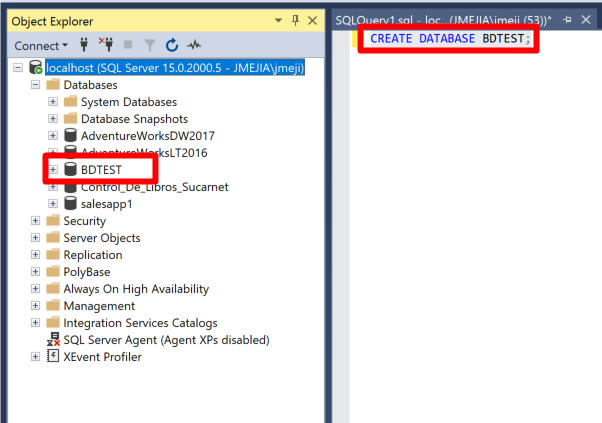
\includegraphics[width=12cm]{./img/1}
	\vspace{2cm}
	\end{center}	
2.  Importamos la  base de datos desde AdventureWorks.
	\begin{center}
	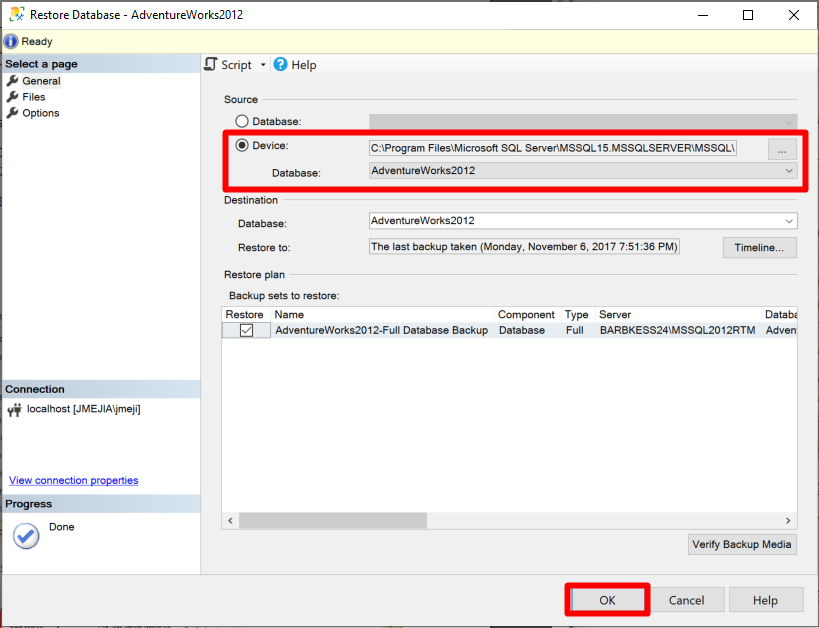
\includegraphics[width=13cm]{./img/2}
	\end{center}	
3. Escribir el Servidor y seleccionar la base de datos
	\begin{center}
	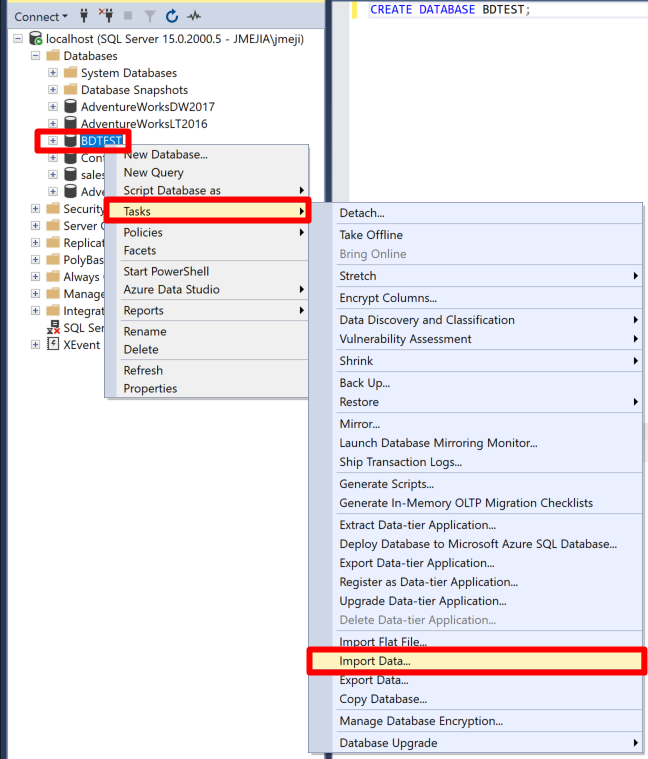
\includegraphics[width=10cm]{./img/3}
	\end{center}	
4. Data Source: La base de donde vamos a importar 
	\begin{center}
	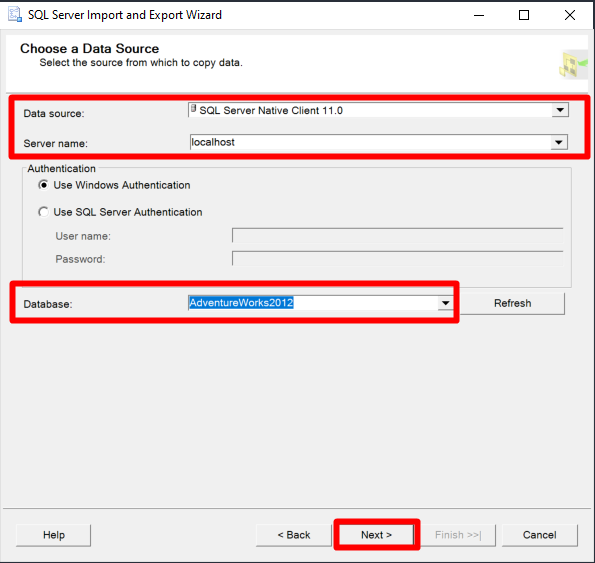
\includegraphics[width=11.5cm]{./img/4}
	\end{center}	
5. Destination: La Base donde vamos a cargar los datos
	\begin{center}
	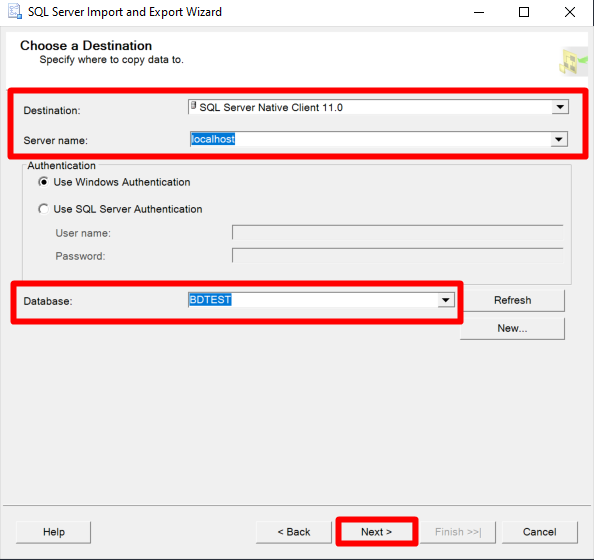
\includegraphics[width=11.5cm]{./img/5}
	\end{center}	
6. Especificar si se realizará copia o consulta, en este caso elejimos copia.
	\begin{center}
	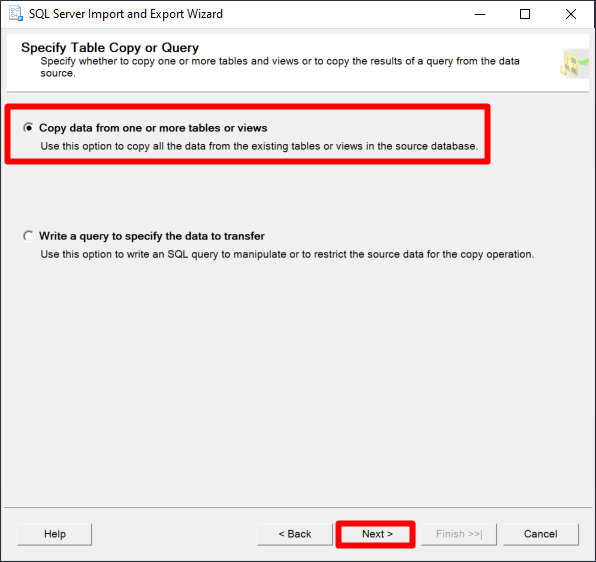
\includegraphics[width=11.5cm]{./img/6}
	\end{center}	
7. Seleccionamos las tablas HumanResources y Person
	\begin{center}
	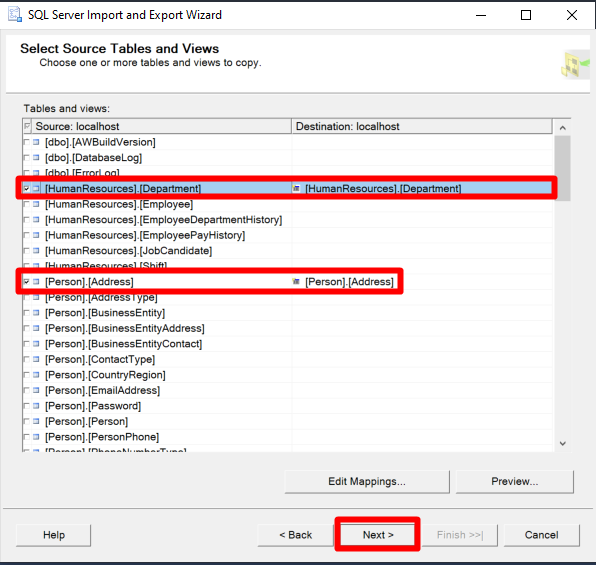
\includegraphics[width=11.5cm]{./img/7}
	\end{center}	
8. Guardamos y ejecutamos.
	\begin{center}
	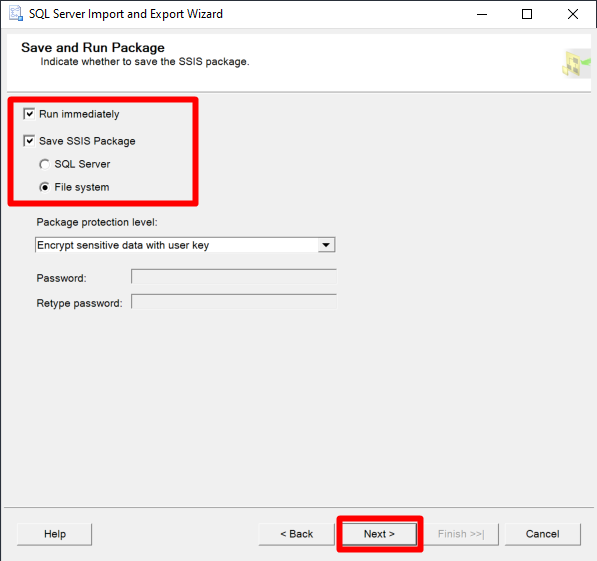
\includegraphics[width=12cm]{./img/8}
	\end{center}	
	\begin{center}
	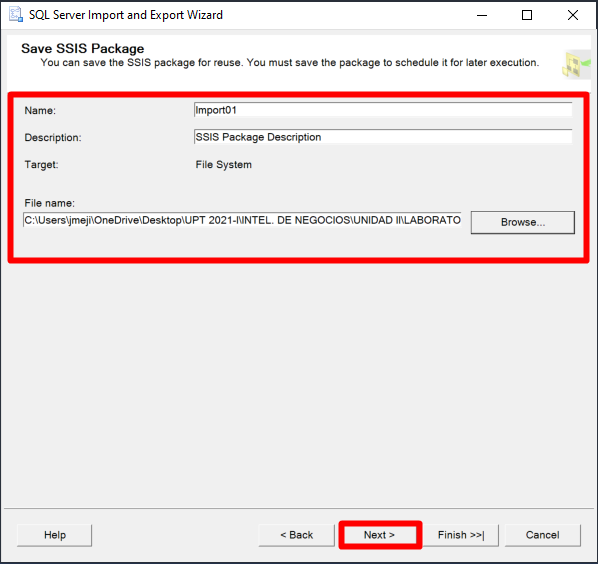
\includegraphics[width=12cm]{./img/9}
	\end{center}	
	\begin{center}
	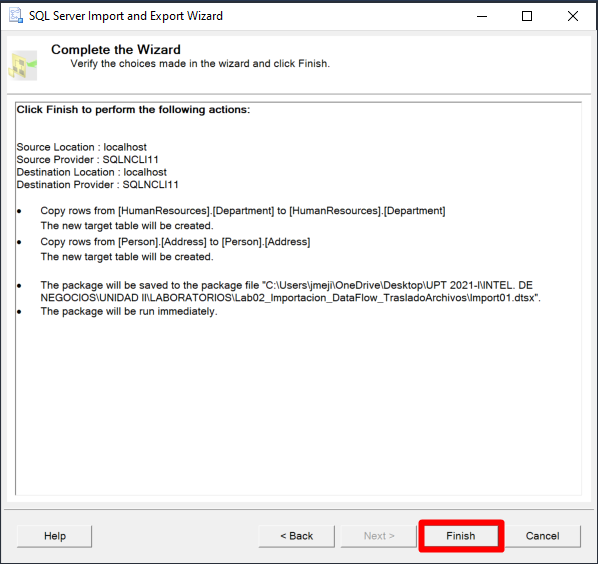
\includegraphics[width=12cm]{./img/10}
	\end{center}		
9. Se observa que se realizó correctamente  la ejecución
	\begin{center}
	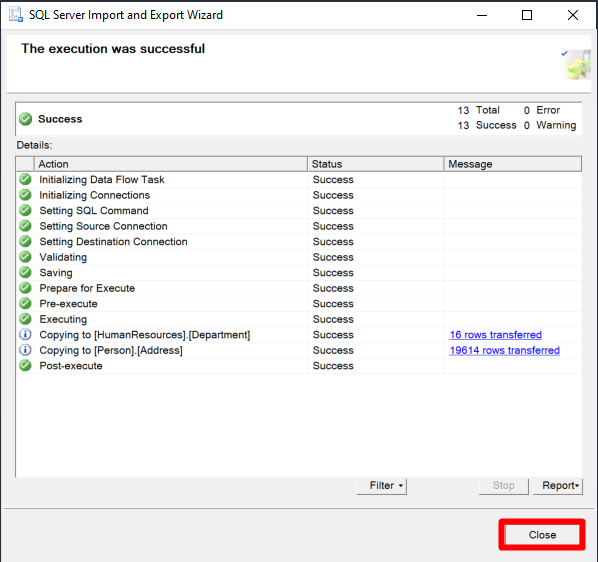
\includegraphics[width=12cm]{./img/11}
	\end{center}	


\subsection{TAREA 2: Creamos Nuestro Primer PAQUETE DTSX}
1.  Abrimos un Nuevo Proyecto en nuestro Visual Basic
	\begin{center}
	
\includegraphics[width=14cm]{./img/12}
	\vspace{2cm}
	\end{center}
	\begin{center}
		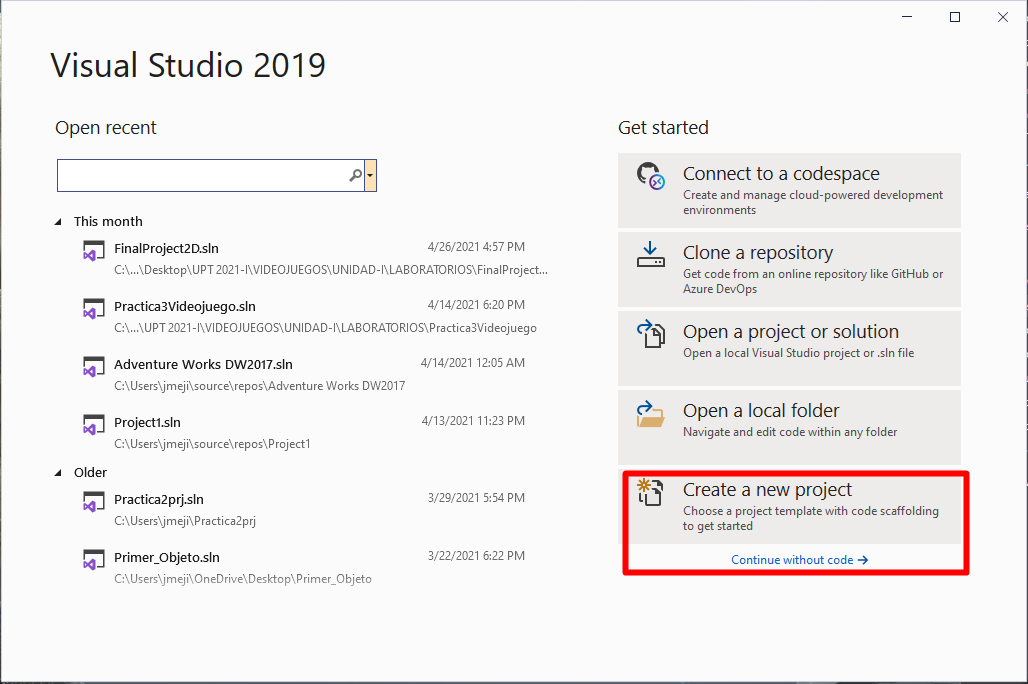
\includegraphics[width=16cm]{./img/13}
	\end{center}
	\begin{center}
		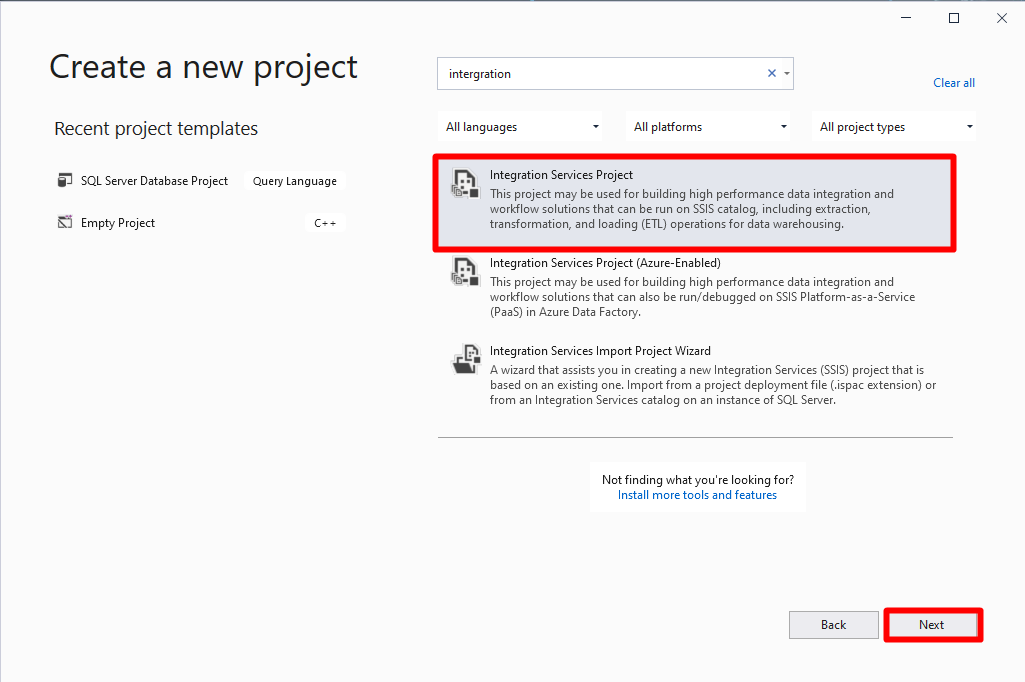
\includegraphics[width=14cm]{./img/14}
	\end{center}	
2.  En la ventana nueva, seccion Solucion Explorer, Agrego el paquete generado antes.
	\begin{center}
	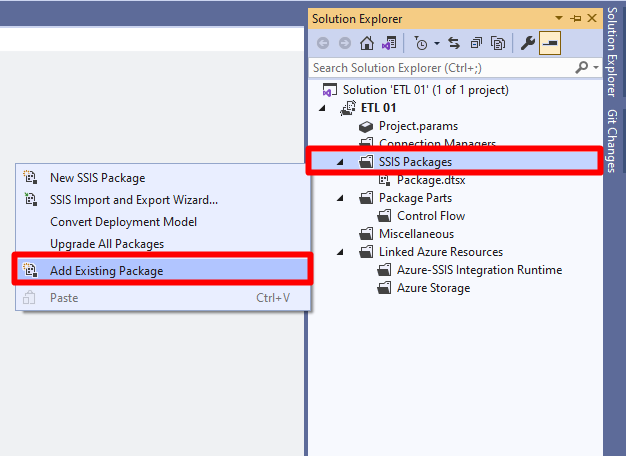
\includegraphics[width=14cm]{./img/15}
	\vspace{2cm}
	\end{center}
	\begin{center}
		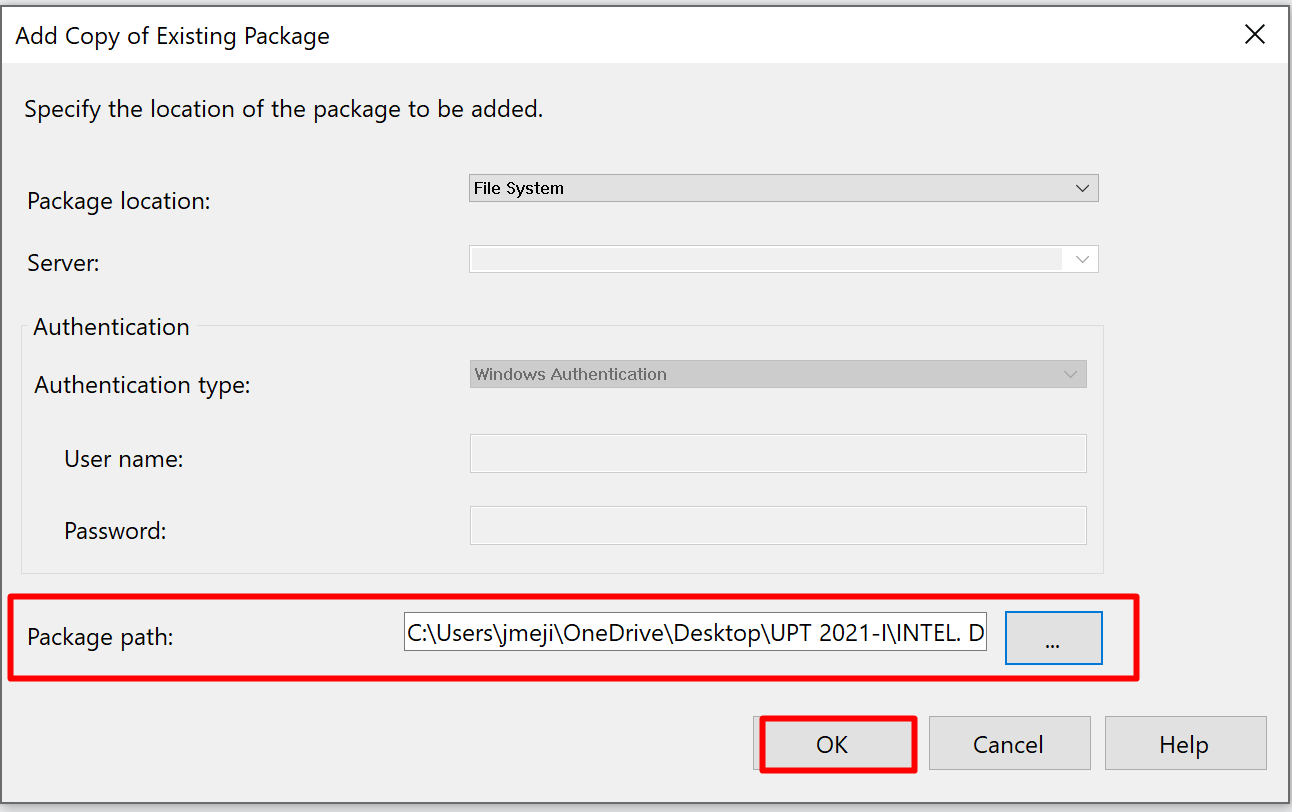
\includegraphics[width=14cm]{./img/16}
		\vspace{2cm}
	\end{center}
	\begin{center}
		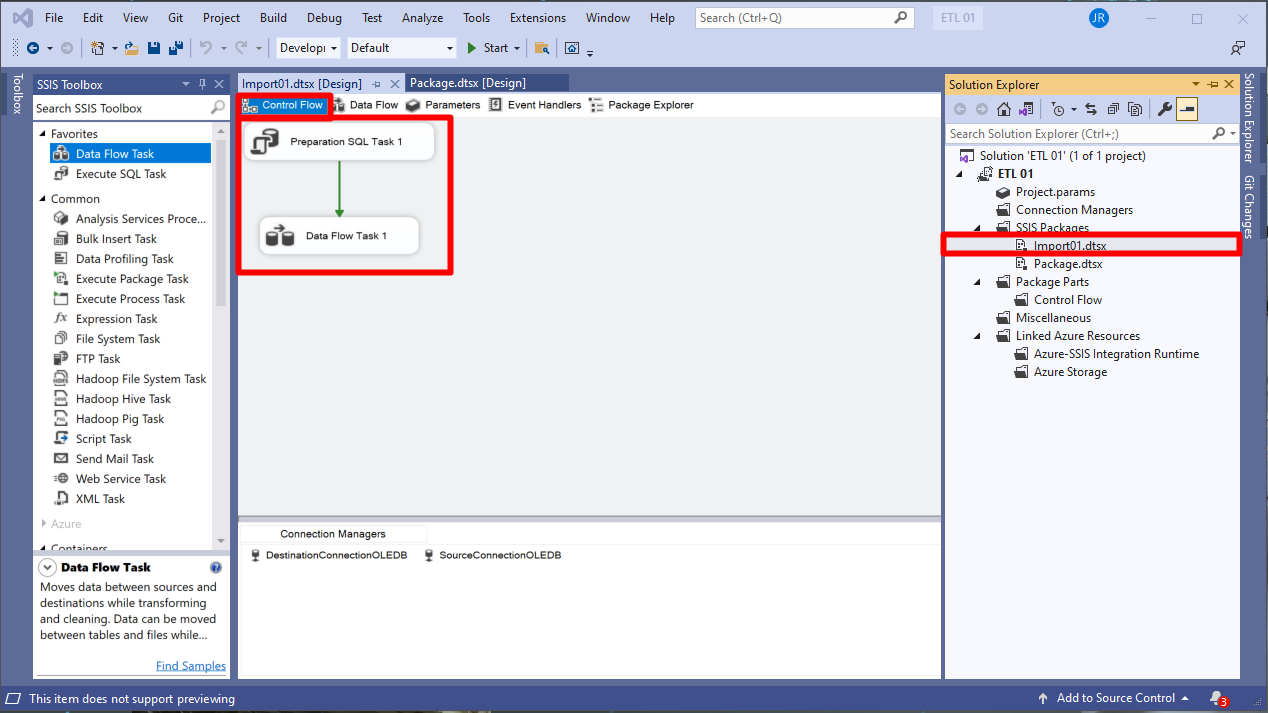
\includegraphics[width=18cm]{./img/17}
		\vspace{2cm}
	\end{center}	
3. Observamos las caracteristicas obtenidas
	\begin{center}
	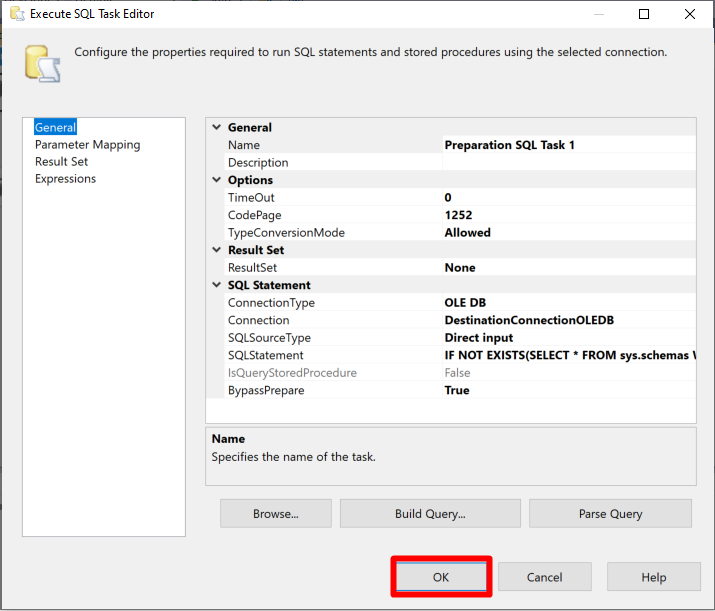
\includegraphics[width=14cm]{./img/18}
	\end{center}	
4. En la siguiente ventana mostramos el paquete que se ha importado.
	\begin{center}
	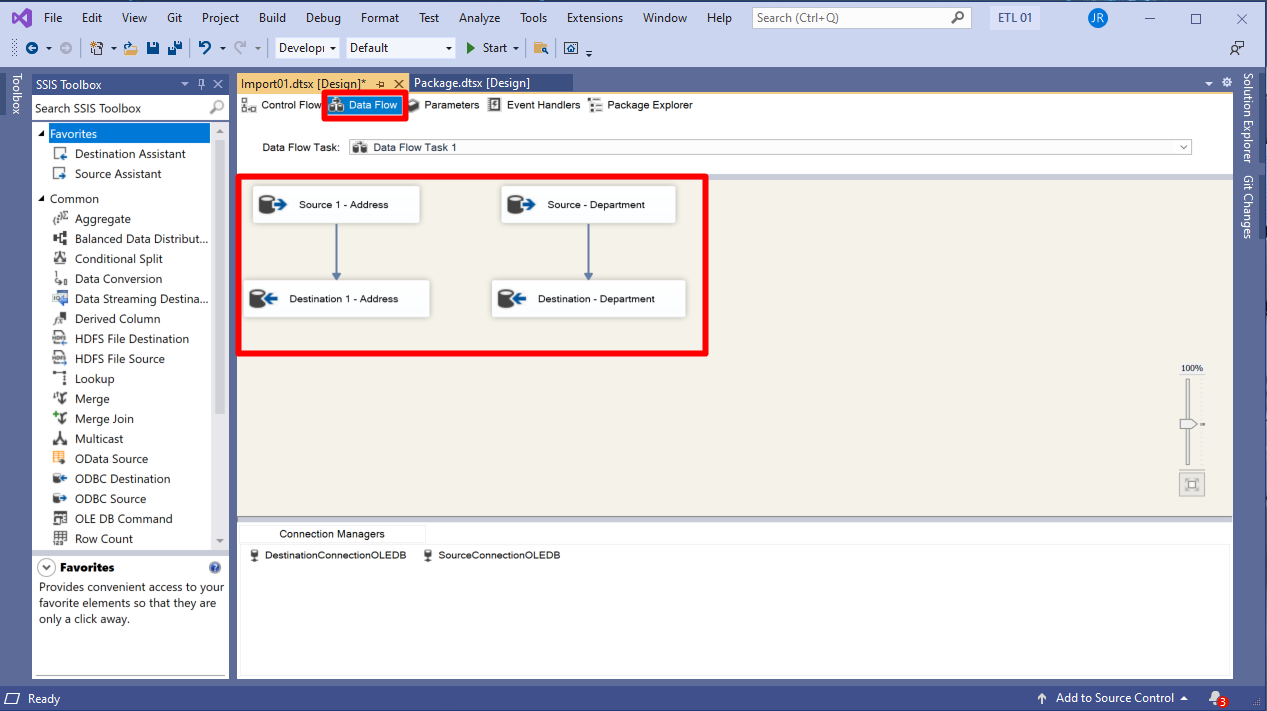
\includegraphics[width=17cm]{./img/19}
	\end{center}
	
\subsection*{MI PRIMER PAQUETE, Muestra la cantidad de Registros de una Tabla}
1. Creacion de Proyecto Intergration Services.
	\begin{center}
	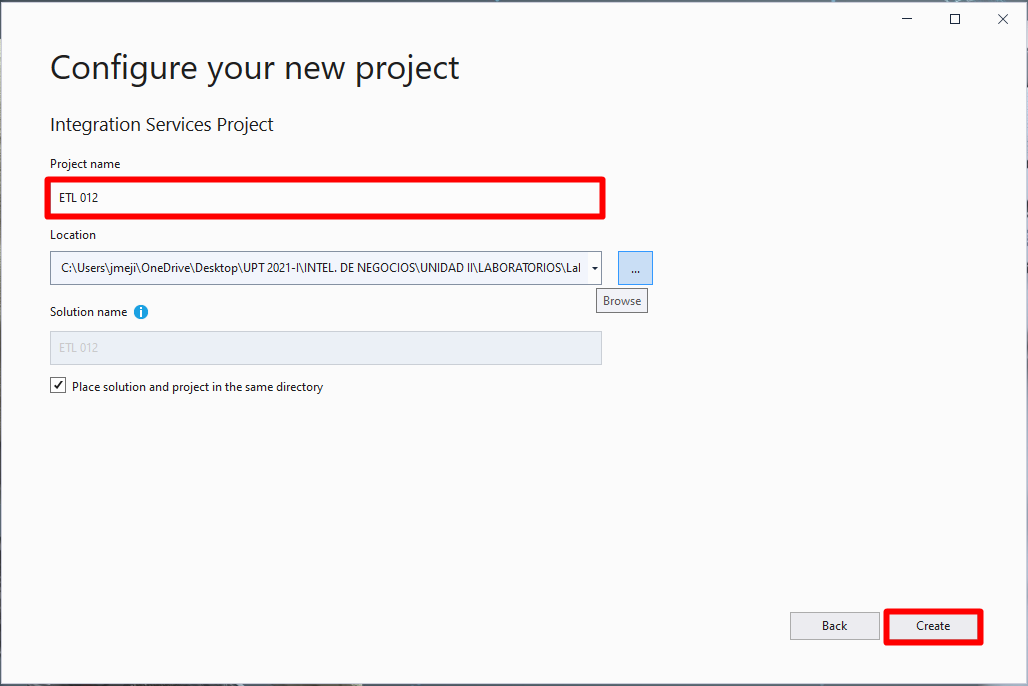
\includegraphics[width=14cm]{./img/27}
	\vspace{2cm}
	\end{center}	
2. Creacion una conexion OLEDB para la base de datos AdventureWorks.
	\begin{center}
	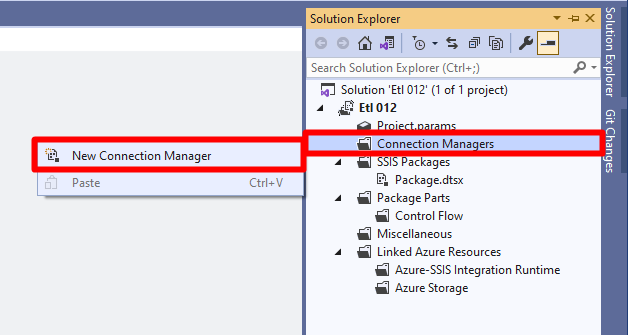
\includegraphics[width=14cm]{./img/28}
	\vspace{2cm}
	\end{center}
3. Seleccion de OLEDB como Driver de Conexion BD 
	\begin{center}
		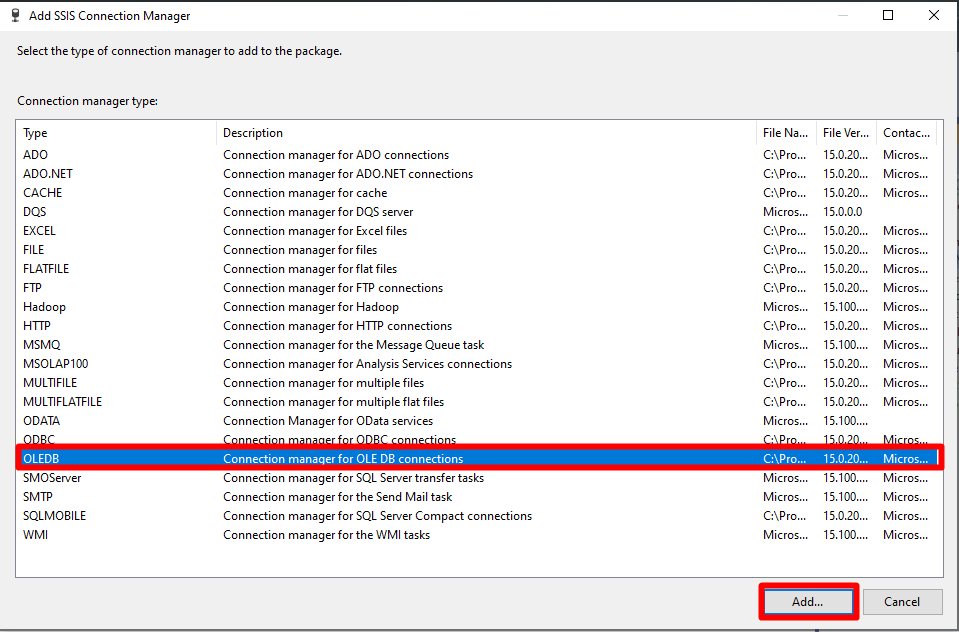
\includegraphics[width=14cm]{./img/29}
		\vspace{2cm}
	\end{center}	
4. Insertar el Server, Base de Datos y Testear.
	\begin{center}
	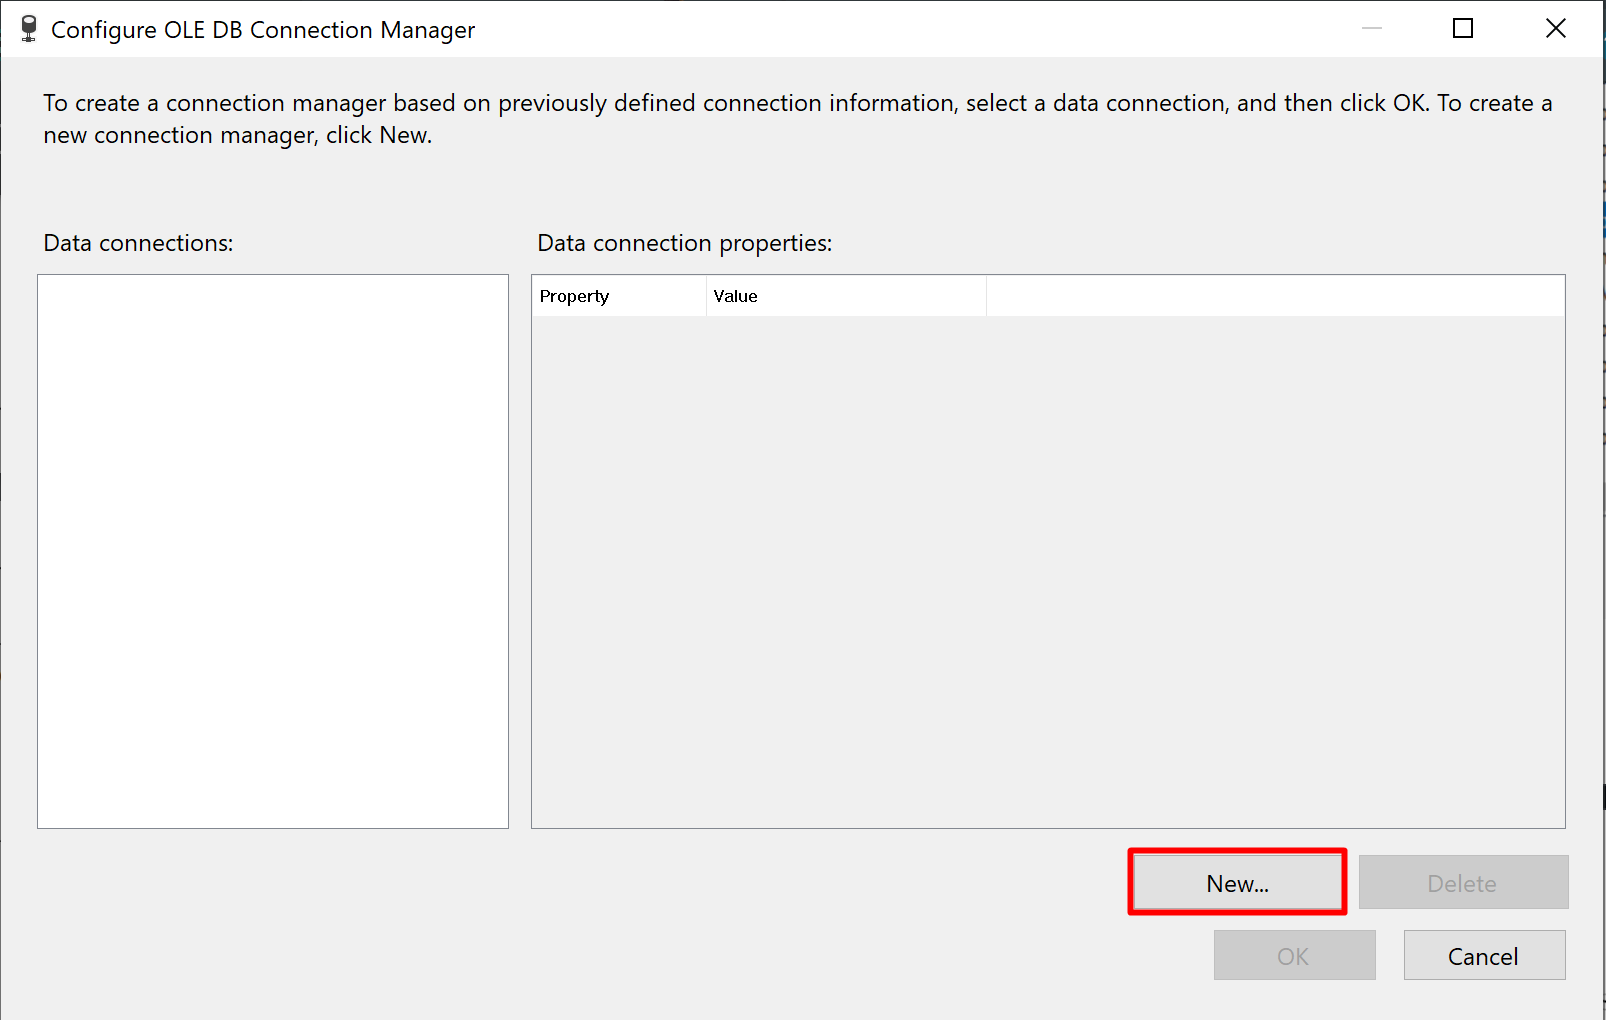
\includegraphics[width=12cm]{./img/22}
	\end{center}
	\begin{center}
		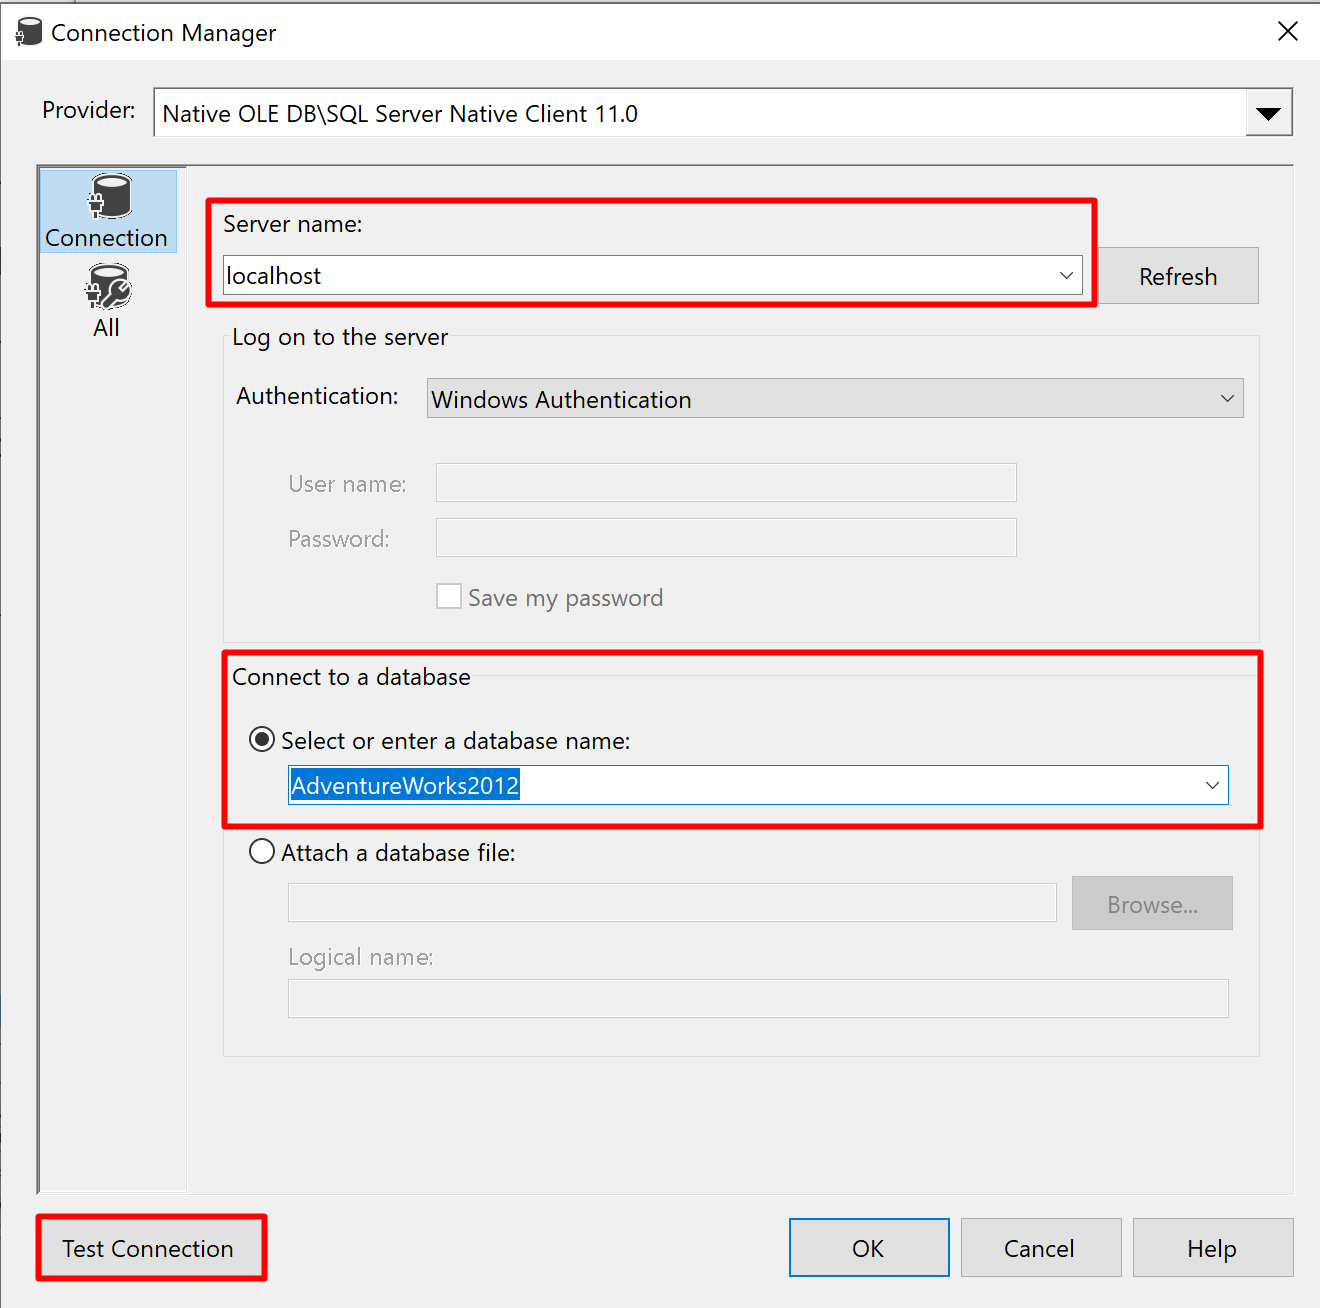
\includegraphics[width=12cm]{./img/23}
	\end{center}
	\begin{center}
		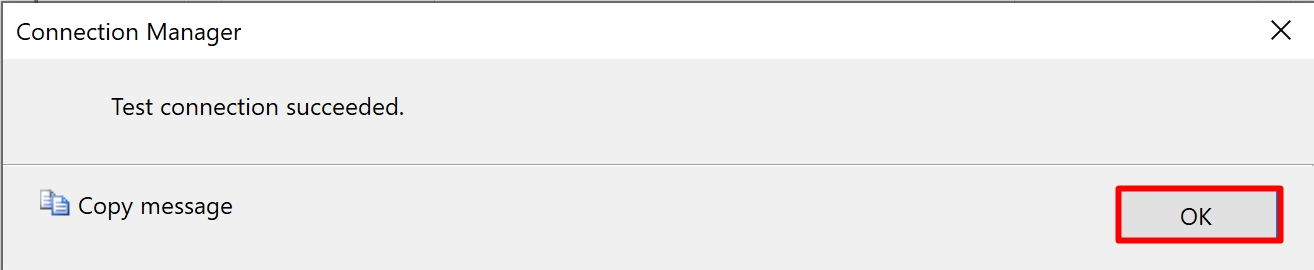
\includegraphics[width=14cm]{./img/24}
	\end{center}
	\begin{center}
		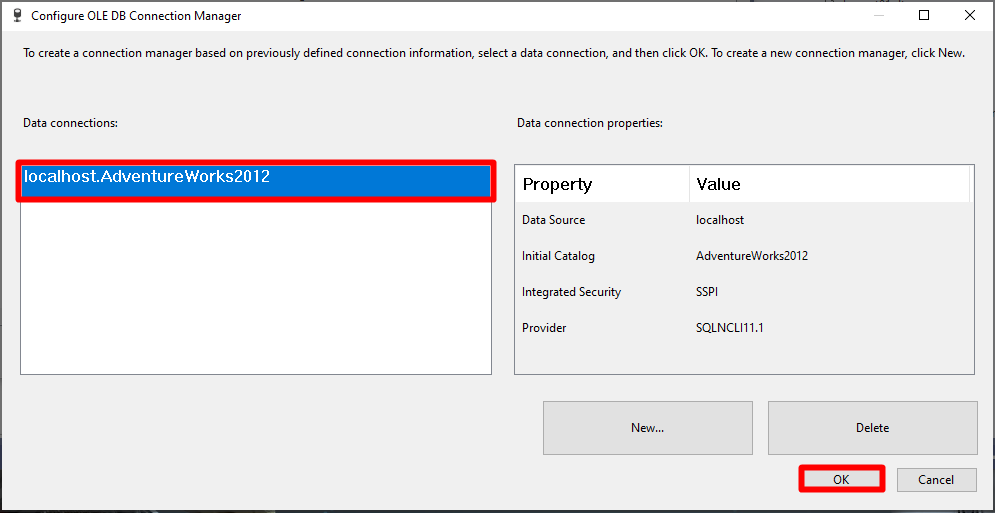
\includegraphics[width=16cm]{./img/25}
	\end{center}
	
\subsection*{Insertar: Execute SQL Task y Script Task}	
1. Insertar los controles, Execute SQL Task Y Script Task.
	\begin{center}
	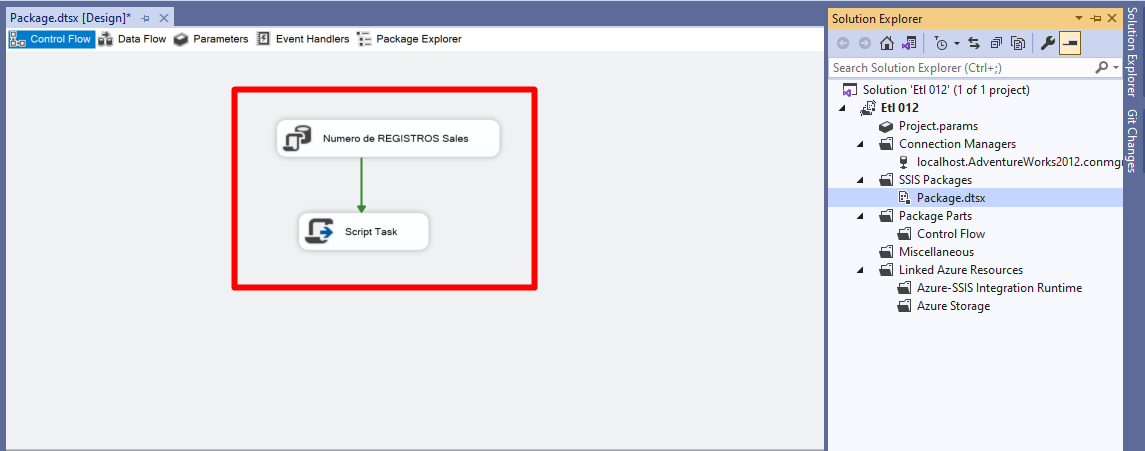
\includegraphics[width=16cm]{./img/34}
	\end{center}
2. Seleccionar:
\\ResultSet = "Single row".
\\ConnectionType="OLE DB" junto con la conexión ya configurada.
\\Digitar la Query.  		
	\begin{center}
	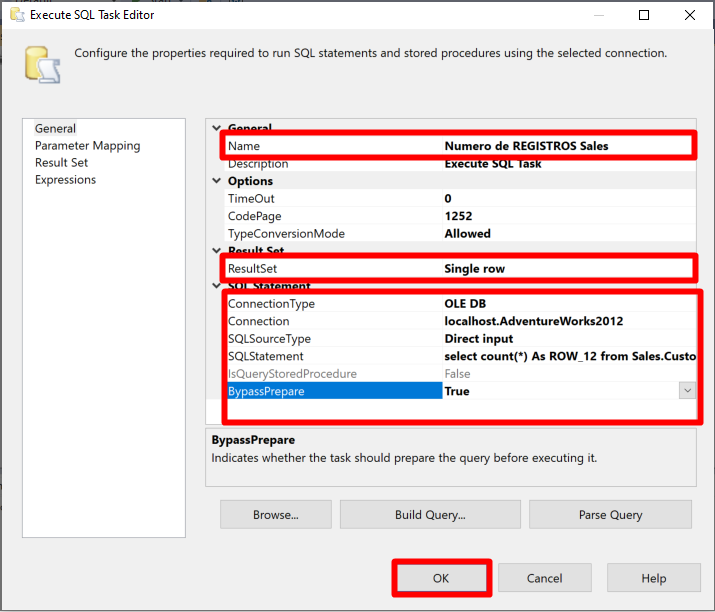
\includegraphics[width=15cm]{./img/32}
	\end{center}
	\begin{center}
		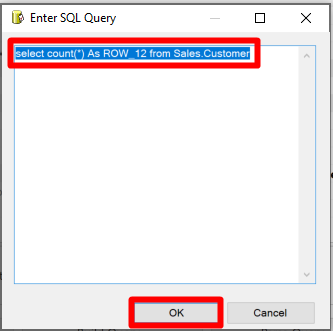
\includegraphics[width=10cm]{./img/33}
		\vspace{2cm}
	\end{center}
3. Crear la Variable.	
	\begin{center}
	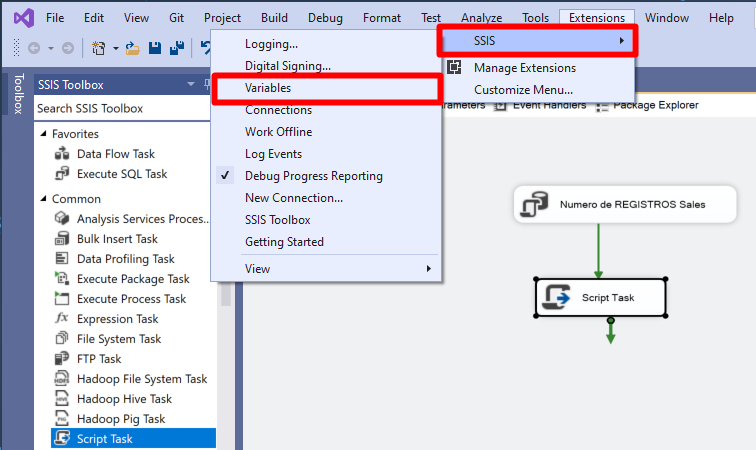
\includegraphics[width=16cm]{./img/35}
	\end{center}
	\begin{center}
		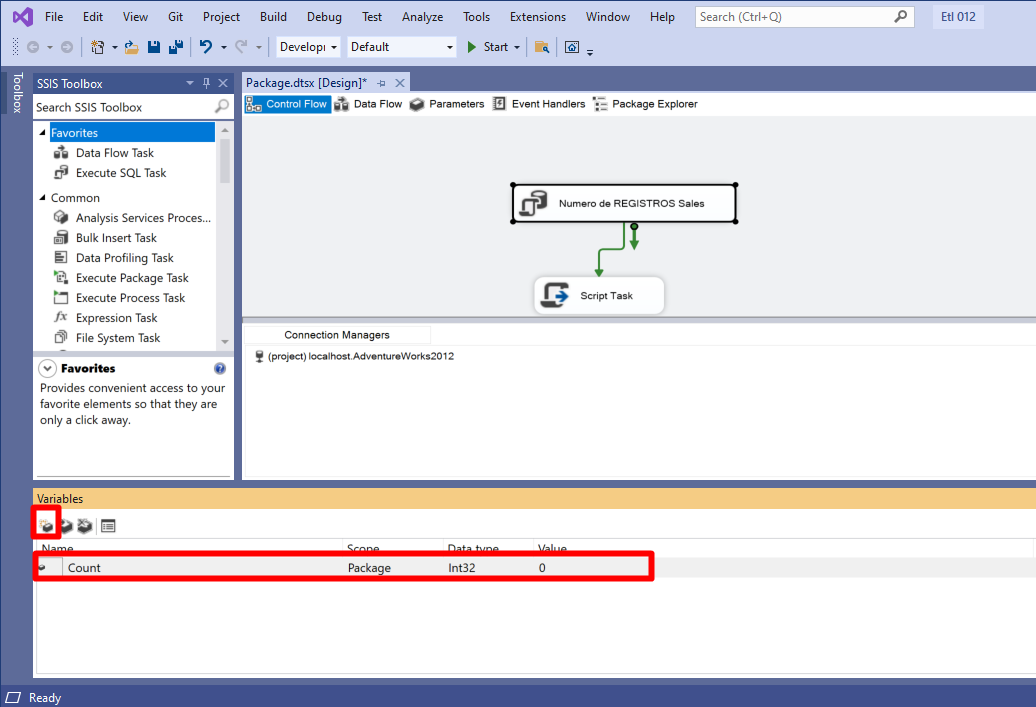
\includegraphics[width=16cm]{./img/36}
	\end{center}		
4. Asignar la variable en “Numero de Registros Sales”.
	\begin{center}
	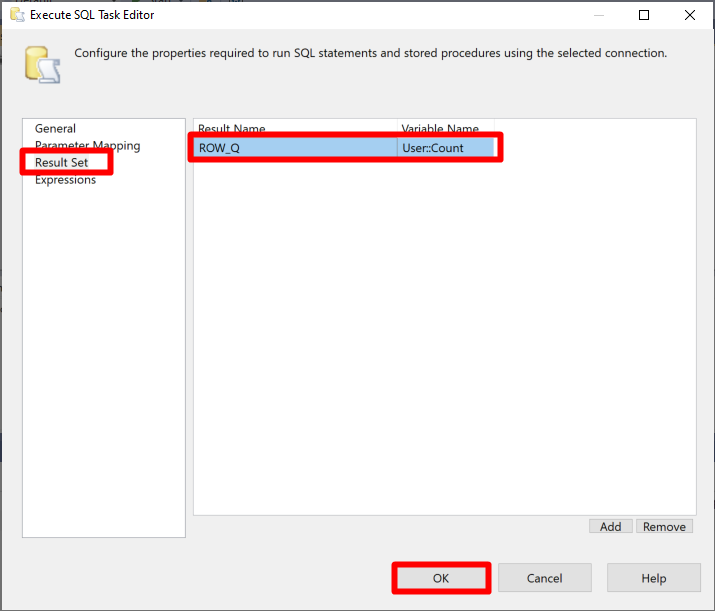
\includegraphics[width=14cm]{./img/38}
	\end{center}
5. EDITAR COMPONENTE “Script Task Editor”
	\begin{center}
	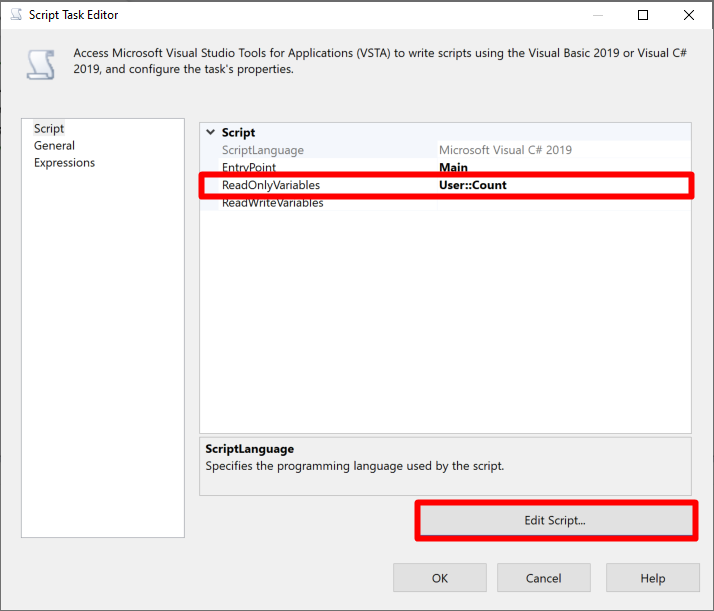
\includegraphics[width=12cm]{./img/39}
	\end{center}
6. Insertar este código “MsgBox(Dts.Variables(0).Value, MsgBoxStyle.Information)”
	\begin{center}
	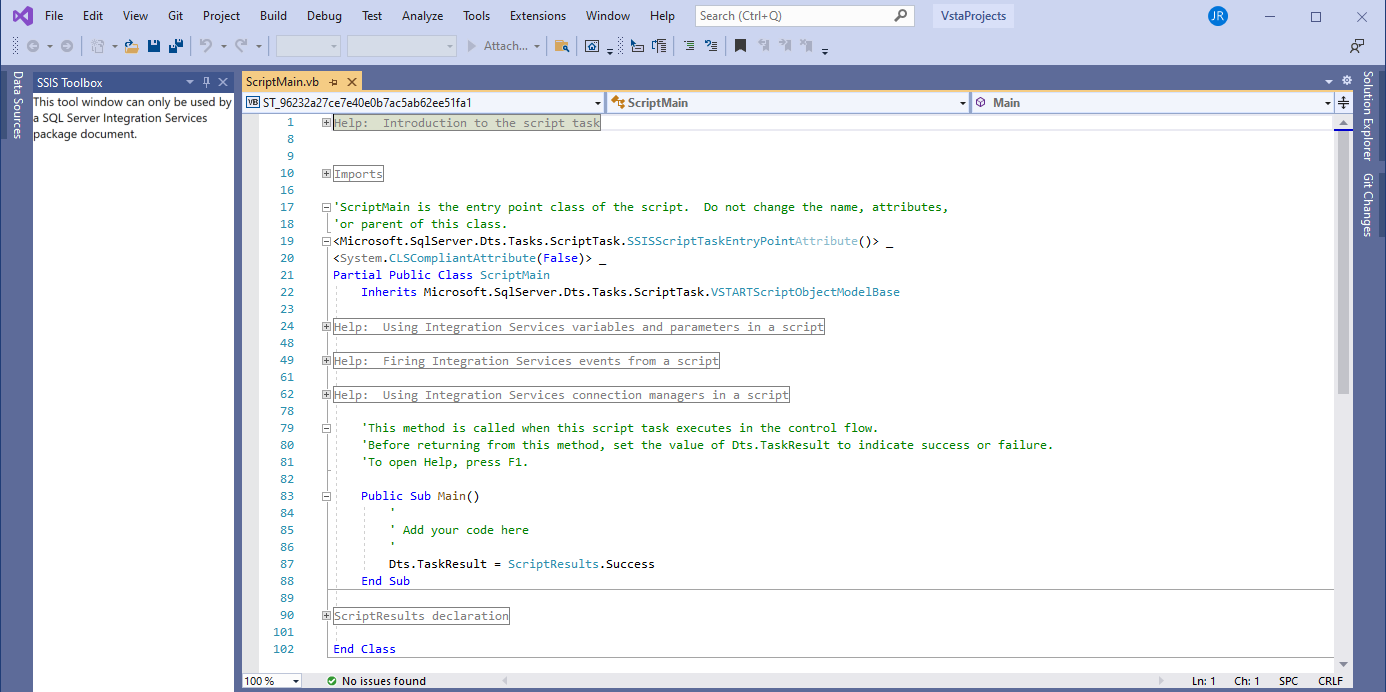
\includegraphics[width=17cm]{./img/40}
	\end{center}
	\begin{center}
	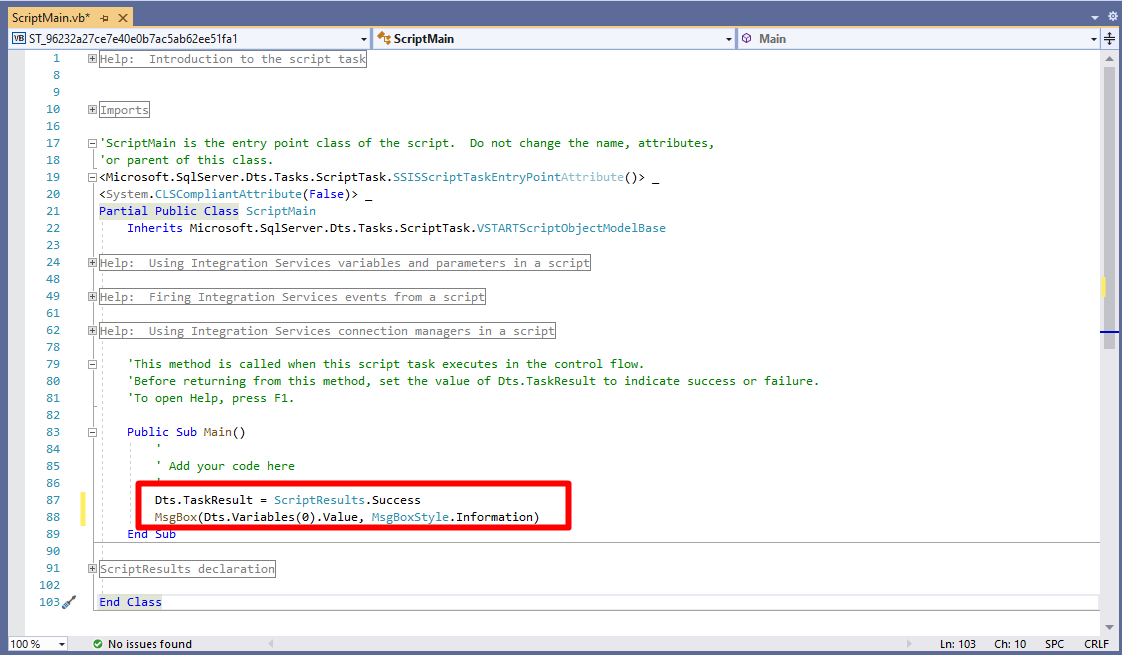
\includegraphics[width=17cm]{./img/41}
	\end{center}
7. Guardamos el proyecto y EJECUTAMOS Y LISTO.
	\begin{center}
	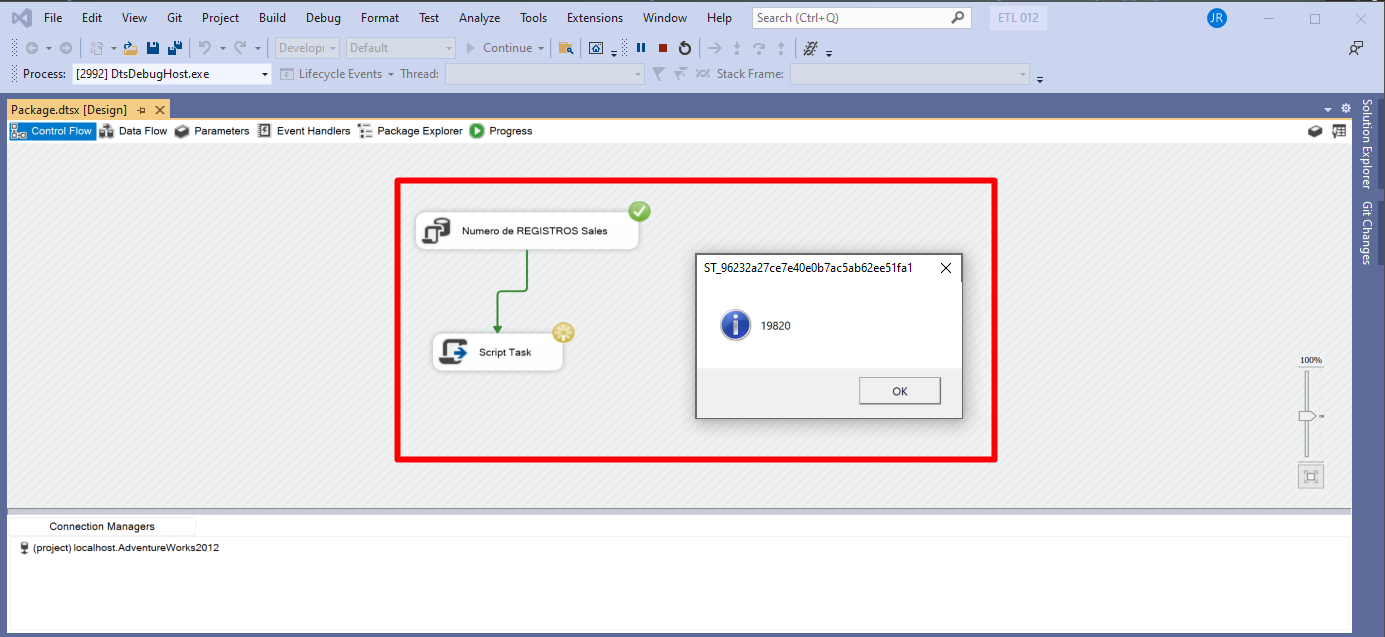
\includegraphics[width=17cm]{./img/42}
	\end{center}
	\begin{center}
	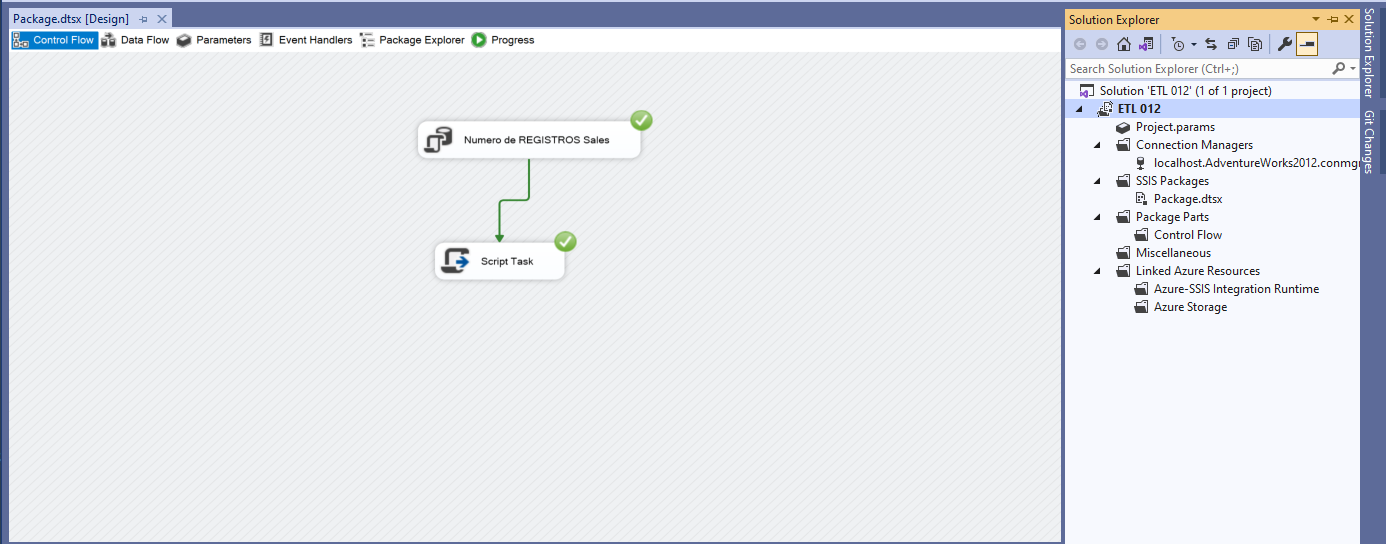
\includegraphics[width=17cm]{./img/43}
	\end{center}
	

\end{document}

